\documentclass[12pt]{article}

\usepackage{sbc-template}

\usepackage{graphicx,url}

\usepackage[brazil]{babel}
%\usepackage[latin1]{inputenc}
\usepackage[utf8]{inputenc}
% UTF-8 encoding is recommended by ShareLaTex


\sloppy

\title{Cai Cai, Passarinho}

\author{Edwino Alberto Lopes Stein\inst{1}, Rafael Sá Menezes\inst{1},
Rodrigo dos Santos Tavares\inst{1}, \\Luciano Ferreira Silva\inst{1} }


\address{Departamento de Ciência da Computação -- Centro de Ciência e Tecnologia
  \\Universidade Federal de Roraima (UFRR)\\
  Boa Vista -- RR -- Brazil
  \email{\{edwino.stein, rafael.sa, rodrigo.tavares\}@ufrr.br, fsluciano.ufrr@gmail.com}
}

\begin{document}

\maketitle

\section{Introdução}
	A computação gráfica é uma das principais áreas da computação, tendo sido muito desenvolvida nas últimas décadas. Com a evolução dela, a área de desenvolvimento de jogos ganhou força, sendo diretamente ligada a evolução da computação gráfica.
	
	Este trabalho irá descrever sobre o jogo \textit{Cai Cai, Passarinho}, desde seu roteiro, mecânicas, artes, até seu desenvolvimento e técnicas utilizadas.
	
\section{Sobre o Jogo}
	O jogo faz uma crítica ao desmatamento, mostrando como uma espécie em extinção pode sobreviver até um certo ponto, mas sempre será extinta, sendo a única maneira de realmente acabar com isso acabar com a fonte do problema (nesse caso, o desmatamento).
\subsection{Roteiro}
	O jogo gira em torno do Passarinho que está fugindo da Máquina Engolidora de Árvores. 
\subsection{Mecânicas do Jogo}
	O jogador deverá mover o Passarinho para os lados, utilizando o acelerômetro, para que ele possa subir de galho em galho e fugir da Máquina Engolidora de Árvores. O objetivo é sobreviver, chegando às alturas mais elevadas. O jogo acaba quando o Passarinho (jogador) não for rápido o suficiente para fugir da Máquina Engolidora de Árvores. Ao acabar, será mostrada a pontuação do jogador e seu recorde atual. Conforme o jogador atinge certos níveis de altura, o nível de dificuldade aumenta, deixando o algoritmo de gerar plataformas com mais peso para plataformas menores e mais distantes.

\section{Arte Gráfica}
\subsection{Cenário}
	O cenário escolhido foi de uma floresta, de dia e sem chuva. A figura~\ref{fig:background} mostra os sprites utilizados, os quais representam diversos fundos se movimentando em velocidades diferentes, criando assim um efeito de profundidade.
	
	\begin{figure}[ht]
		\centering
		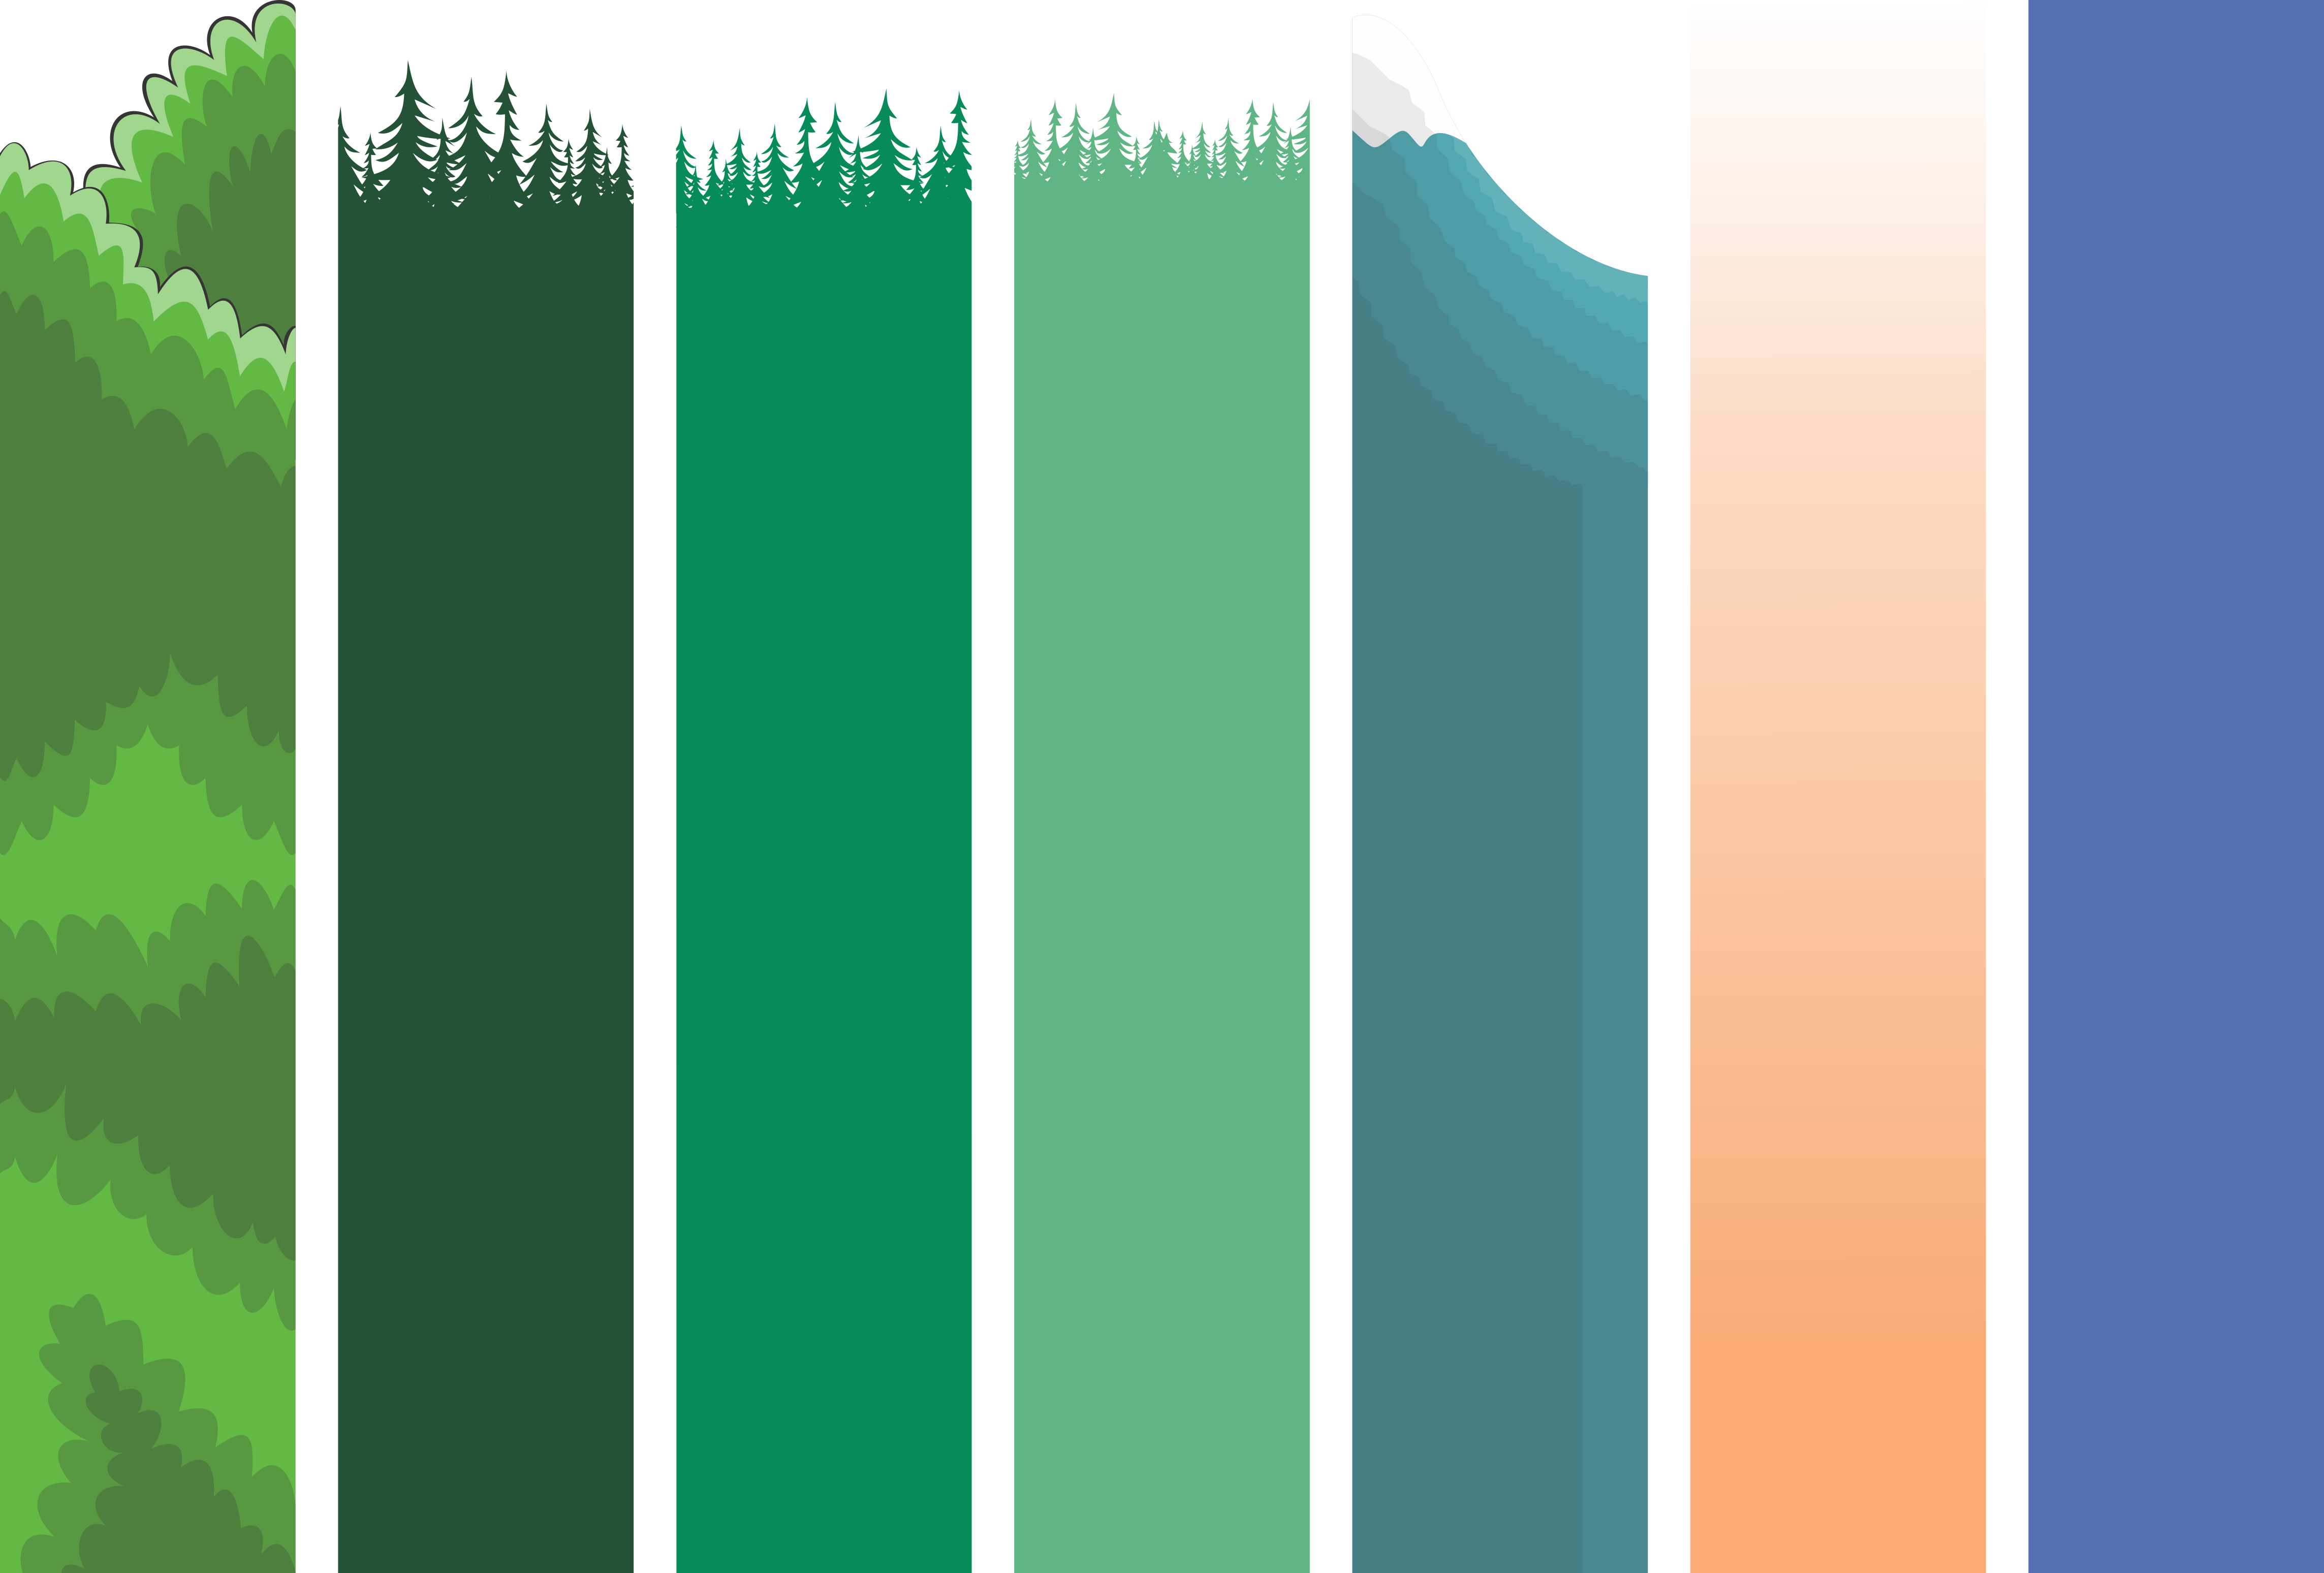
\includegraphics[width=.5\textwidth]{imagens/Background}
		\caption{Background}
		\label{fig:background}
	\end{figure}
	
	A figura \ref{fig:tronco} mostra o sprite do tronco da árvore, o qual fica se replicando conforme o jogador atinge novas alturas. 	
	\begin{figure}[ht]
		\centering
		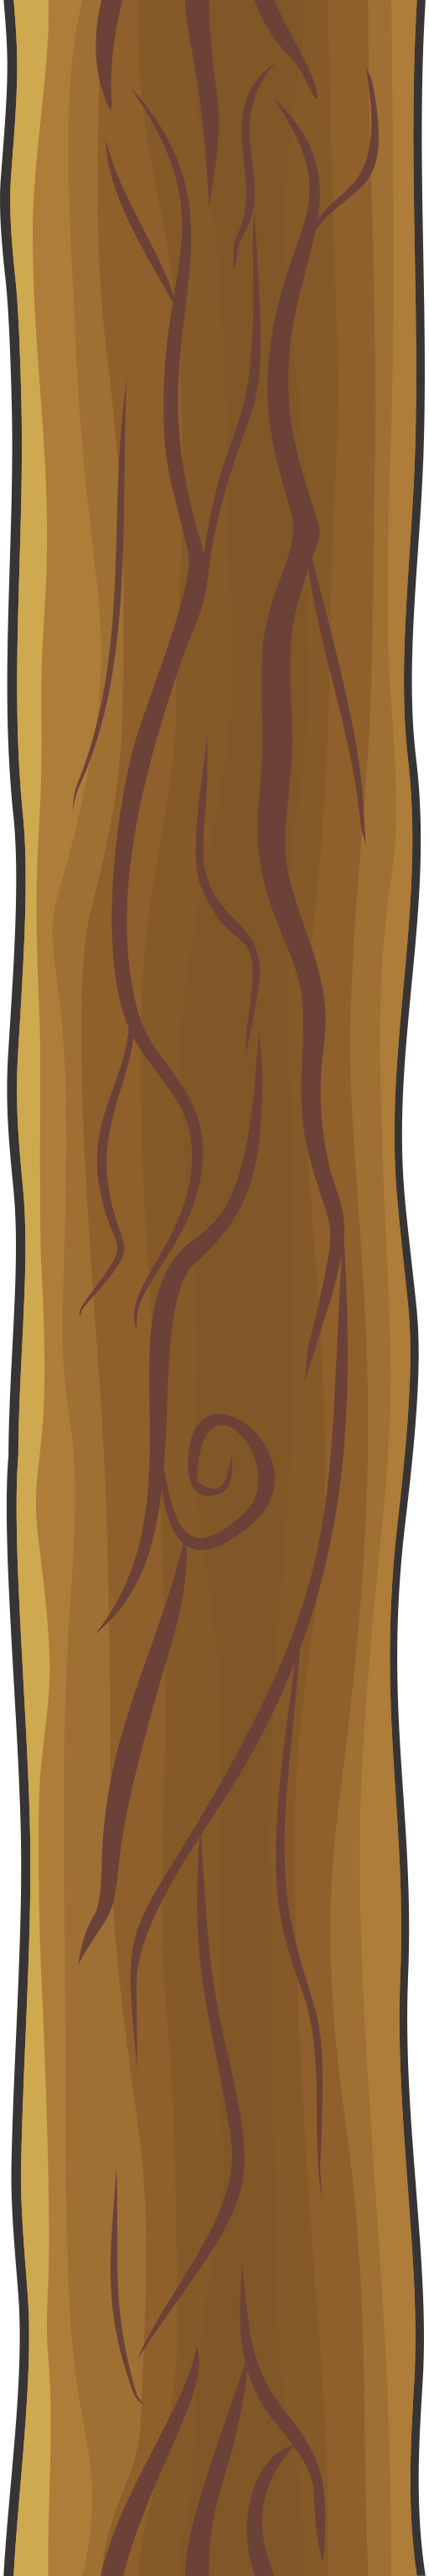
\includegraphics[height=5cm]{imagens/Bole}
		\caption{Tronco da árvore}
		\label{fig:tronco}
	\end{figure}
	
	A figura \ref{fig:galho} mostra o sprite do galho, que sai do tronco e se alinha automaticamente a alguma plataforma.
	\begin{figure}[ht]
		\centering
		
\includegraphics[height=2cm]{imagens/branch}
		\caption{Galho da árvore}
		\label{fig:galho}
	\end{figure}

	A figura \ref{fig:plataforma} mostra o sprite da plataforma, que pode ser dividida em três tamanhos: pequeno (1 unidade), médio (2 unidades) e grande (3 unidades).
	\begin{figure}[ht]
		\centering
		
\includegraphics[height=2cm]{imagens/Platform2}
		\caption{Plataforma}
		\label{fig:plataforma}
	\end{figure}
			
\subsection{Personagens}
	O personagem principal do jogo é ilustrado pela figura~\ref{fig:passarinho}.	A figura~\ref{fig:maq} exibe o sprite da Máquina Engolidora de Árvores. A figura~\ref{fig:saw} mostra o sprite da serra da máquina.
	
	\begin{figure}[ht]
		\centering
		
\includegraphics[width=.5\textwidth]{imagens/Player}
		\caption{Passarinho}
		\label{fig:passarinho}
	\end{figure}
	
	\begin{figure}[ht]
		\centering
		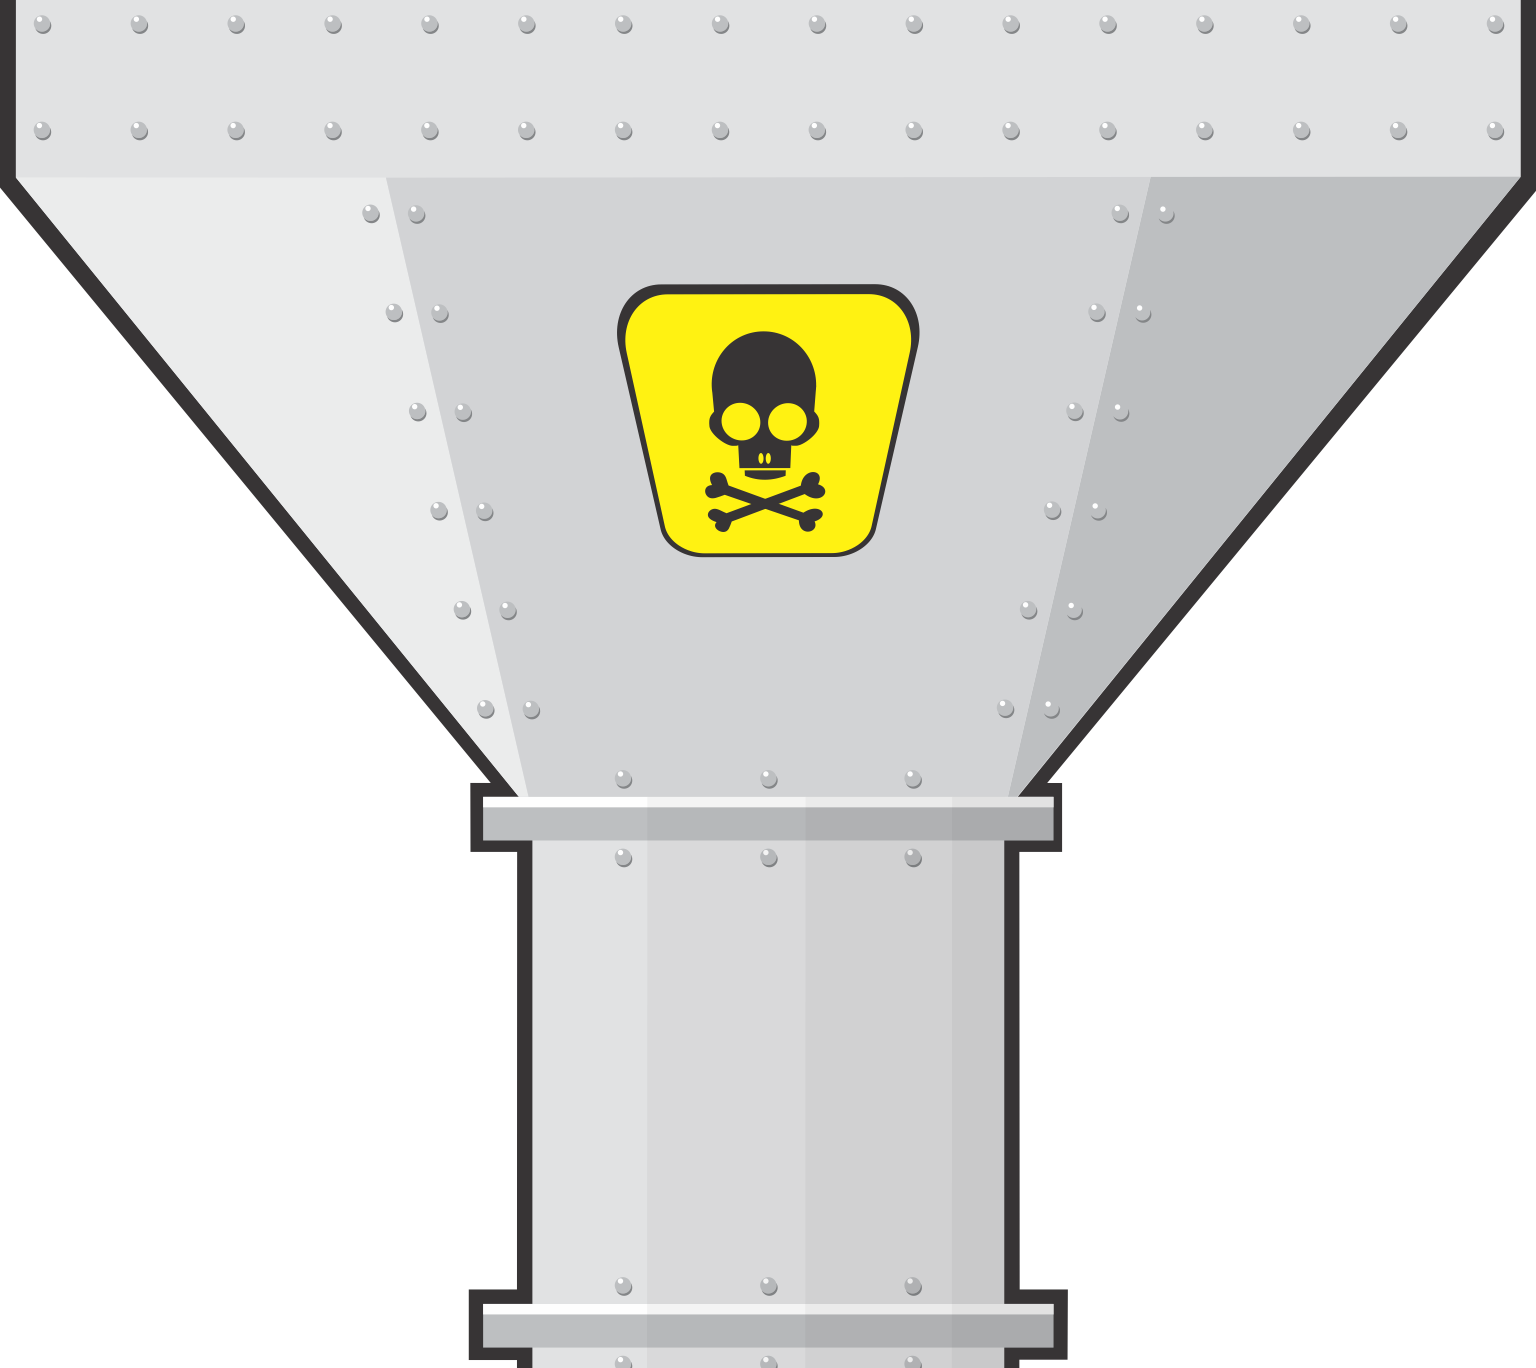
\includegraphics[width=.5\textwidth]{imagens/Machine}
		\caption{Máquina Engolidora de Árvores}
		\label{fig:maq}
	\end{figure}
			
	\begin{figure}[ht]
		\centering
		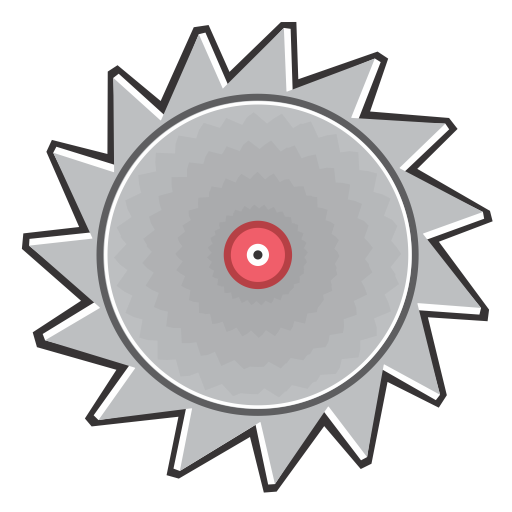
\includegraphics[width=.5\textwidth]{imagens/Saw}
		\caption{Serra}
		\label{fig:saw}
	\end{figure}
\section{Desenvolvimento}
\subsection{Ferramentas de Desenvolvimento}
	As ferramentas utilizadas durante o desenvolvimento foram:
	
	\begin{description}
		\item [Unity:] Para desenvolvimento do jogo.
		\item [Corel Draw:] Para criação dos sprites.
	\end{description}

%\subsection{Menus}
%\subsection{Física}
%\subsection{Ações}
\subsection{Pontuação}
	O jogo utiliza um sistema de pontuação que conta os pontos baseado na altura máxima atingida. Ao final da partida, o jogo exibe para o jogador a maior pontuação já obtida e sua pontuação atual.
\subsection{Técnicas Utilizadas}

\subsubsection{Gerador de plataformas}
	Para geração das plataformas, foi utilizado um algoritmo próprio que funciona da seguinte forma:
	\begin{enumerate}
		\item Separa o cenário em 14 colunas de tamanhos iguais;
		\item Define a regra para criação de cada linha de plataforma;
		\item Ao iniciar o jogo, são geradas algumas plataformas próximas ao jogador, de forma que garanta que ele morra no início do jogo.
		\item Ao começar a subir, é inicializado o algoritmo de geração.
		\item A cada linha, as plataformas são geradas baseadas no nível atual (que define possibilidade de geração, distância e tamanho).		
		\item Ao gerar as plataformas, verifica se o jogador consegue alcançar as próximas plataformas (baseando-se na distância do pulo do Passarinho), senão gera uma nova plataforma acessível.
	\end{enumerate}

\subsection{Algoritmos Clássicos}
 	Para a exibição do cenário, a câmera utilizaou algoritmos de recorte. Durante a criação das sprites, foi utilizado Curvas de Bézier para deixa-las mais suaves. Durante o \textit{gameplay} são utilizadas transformações nos movimentos dos personagens.

\section{Conclusão}
	Neste trabalho foi apresentado o jogo \textit{Cai, Cai Passarinho}, um \textit{infinity run} onde tenta se subir o maior número possíveis de plataformas sem encostar na máquina. O jogo foi desenvolvido para Android utilizando Unity e Corel Draw e tenta passar uma crítica sobre o desmatamento.

\end{document}
